\chapter{Results}

\section{Segmented Audio Signal}

The audio signal was successfully segmented into individual notes based on the manually selected time splits. Each segment corresponds to a distinct note played by the music box. As seen in \autoref{fig:time_plot_segment_1}, the waveform of Segment 1 clearly shows the onset and decay of the note, and shows that the note is allowed to die out before another note occurs. This segmentation allows for isolated analysis of each note's frequency content.

\begin{figure}[H]
    \centering
    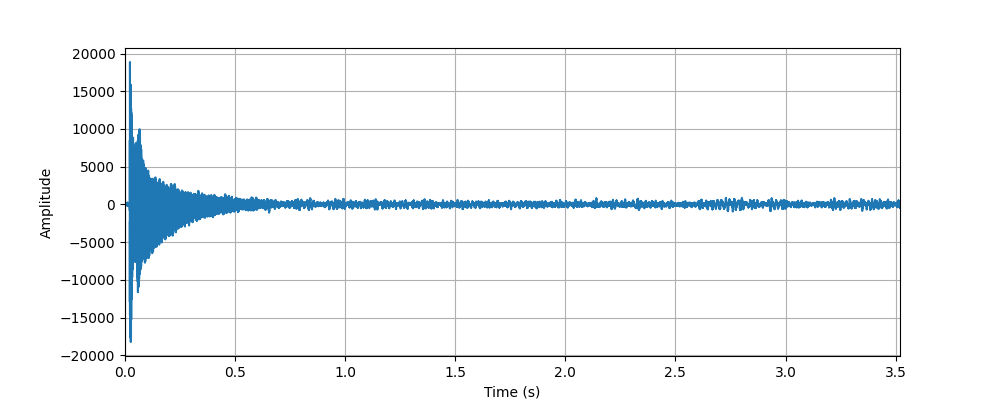
\includegraphics[width=\textwidth]{data/time_plots/time_plot_segment_1.png}
    \caption{Waveform of Segment 1}
    \label{fig:time_plot_segment_1}
\end{figure}


\section{FFT Analysis of Music Box Recording}

\subsection{Segmented FFT Analysis}

For each segment, the frequency resolution was calculated using \autoref{eq:freq_resolution}, taking into account the zero-padding applied to each segment. A frequency resolution of approximately 0.04 Hz was achieved for all segments after zero-padding. 

If we look at the FFT of Segment 1 in \autoref{fig:fft_segment_1}, we can see that the fundamental frequency is approximately 1106.56 Hz. 

\begin{figure}[H]
    \centering
    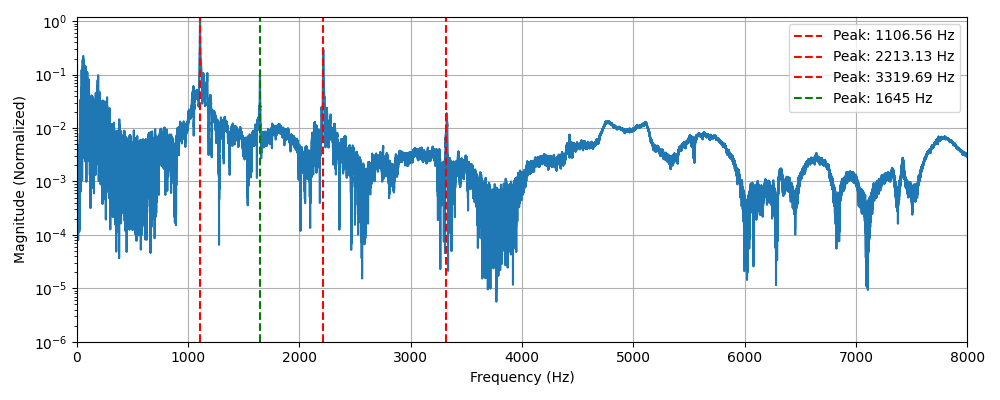
\includegraphics[width=\textwidth]{data/fft_spectrums/fft_spectrum_segment_1.png}
    \caption{FFT of Segment 1 with identified peaks}
    \label{fig:fft_segment_1}
\end{figure}

\subsection{Overharmonic Peaks Identification}

Also as seen in \autoref{fig:fft_segment_1}, the harmonic peaks are identified by looking for peaks in the FFT magnitude spectrum that are integer multiples of the fundamental frequency. These are classified as Group A peaks, since they are harmonic to the fundamental frequency. 

The Group B peaks, which are not harmonic to the fundamental frequency, are also identified in \autoref{fig:fft_segment_1}. These peaks do not correspond to integer multiples of the fundamental frequency and are likely due to other resonances or noise in the recording. The peak at approximately 1645 Hz is an example of a Group B peak. There is also a peak closer to 60 Hz, which is likely due to noise from the surrounding environment.

The deviation of the actual harmonic peaks from the perfect harmonic frequencies is calculated in cents and is summarized in Table \ref{tab:deviation_segment_1}. 

\begin{table}[H]
    \centering
    \caption{Deviation of Harmonic Peaks from Perfect Harmonics for Segment 1}
    \begin{tabular}{ccc}
        \hline
        Harmonic & Actual Frequency (Hz) & Deviation (cents) \\
        \hline
        1st (Fundamental) & 1106.56 & 0 \\
        2nd & 2213.12 & 0 \\
        3rd & 3319.68 & -5.85 \\
        4th & 4426.25 & -11.73 \\
        \hline
    \end{tabular}
    \label{tab:deviation_segment_1}
\end{table}

The amplitudes of the harmonic peaks relative to the fundamental frequency are summarized in \autoref{tab:harmonic_amplitudes_segment_1}. 

\begin{table}[H]
\centering
\caption{Harmonic Amplitudes in dB relative to Fundamental for Segment 1}
\begin{tabular}{|c|c|c|}
\hline
Harmonic & Frequency (Hz) & dB (relative to fundamental) \\
\hline
1 & 1106.56 & 0 \\
2 & 2213.12 & -10.51 \\
3 & 3319.68 & -34.54 \\
4 & 4426.25 & -42.48 \\
\hline
\end{tabular}
\label{tab:harmonic_amplitudes_segment_1}
\end{table}


\section{Note Identification and Melody Extraction}

Using \autoref{eq:note_freq}, the identified peak frequencies were mapped to their corresponding musical notes. The notes were then categorized into melody and bass based on their frequencies. Notes above middle C (approximately 261.63 Hz) were classified as melody, while those below were classified as bass.

The melody frequencies and their corresponding notes are summarized in \autoref{tab:melody_freq_notes}. Also the deviation in cents from the ideal frequency is included in this table.

\begin{table}[H]
    \centering
    \caption{Identified Melody Frequencies, Corresponding Notes, and Deviation in Cents}
    \begin{tabular}{cccc}
        \hline
        Segment & Frequency (Hz) & Note & Deviation (cents) \\
        \hline
        1  & 1106.56 & C\#6  & -3.39   \\
        3  & 1174.57 & D6    & -0.13   \\
        5  & 1319.50 & E6    & 1.30    \\
        6  & 1401.42 & F6    & 5.58    \\
        7  & 591.87  & D5    & 13.33   \\
        8  & 1105.89 & C\#6  & -4.44   \\
        10 & 1171.75 & D6    & -4.29   \\
        11 & 1319.41 & E6    & 1.19    \\
        12 & 1396.42 & F6    & -0.61   \\
        13 & 1863.25 & A\#6  & -1.30   \\
        15 & 591.91  & D5    & 13.45   \\
        16 & 1767.40 & A6    & 7.27    \\
        17 & 1174.57 & D6    & -0.13   \\
        18 & 1401.38 & F6    & 5.53    \\
        19 & 1751.76 & A6    & -8.12   \\
        20 & 1171.62 & D6    & -4.48   \\
        21 & 1656.67 & G\#6  & -4.75   \\
        22 & 5145.13 & E8    & -42.84  \\
        25 & 1562.33 & G6    & -6.25   \\
        26 & 1396.63 & F6    & -0.35   \\
        27 & 1173.52 & D6    & -1.68   \\
        28 & 1047.30 & C6    & 1.33    \\
        29 & 1171.67 & D6    & -4.42   \\
        30 & 470.87  & A\#4  & 17.39   \\
        31 & 591.91  & D5    & 13.45   \\
        33 & 1106.44 & C\#6  & -3.59   \\
        34 & 1174.57 & D6    & -0.13   \\
        36 & 1319.46 & E6    & 1.24    \\
        37 & 1770.05 & A6    & 9.86    \\
        38 & 1401.30 & F6    & 5.43    \\
        39 & 591.91  & D5    & 13.45   \\
        40 & 1106.14 & C\#6  & -4.05   \\
        41 & 1171.79 & D6    & -4.23   \\
        42 & 699.70  & F5    & 3.09    \\
        43 & 1319.41 & E6    & 1.19    \\
        44 & 1396.34 & F6    & -0.72   \\
        45 & 1863.55 & A\#6  & -1.03   \\
        46 & 591.87  & D5    & 13.33   \\
        47 & 1757.56 & A6    & -2.40   \\
        49 & 1401.26 & F6    & 5.37    \\
        50 & 1767.24 & A6    & 7.10    \\
        51 & 1767.53 & A6    & 7.39    \\
        52 & 2337.53 & D7    & -8.71   \\
        53 & 470.83  & A\#4  & 17.24   \\
        54 & 1106.60 & C\#6  & -3.32   \\
        55 & 1562.38 & G6    & -6.20   \\
        56 & 2211.57 & C\#7  & -4.61   \\
        \hline
    \end{tabular}
    \label{tab:melody_freq_notes}
\end{table}

The bass frequencies and their corresponding notes are summarized in \autoref{tab:bass_freq_notes}. 

\begin{table}[H]
    \centering
    \caption{Identified Bass Frequencies, Corresponding Notes, and Deviation in Cents}
    \begin{tabular}{cccc}
        \hline
        Segment & Frequency (Hz) & Note & Deviation (cents) \\
        \hline
        2  & 53.20  & G\#1  & +42.46 \\
        4  & 86.85  & F2    & -9.13  \\
        9  & 53.83  & A1    & -37.13 \\
        14 & 56.31  & A1    & +40.89 \\
        23 & 57.11  & A\#1  & -34.72 \\
        24 & 59.26  & A\#1  & +29.10 \\
        32 & 76.80  & D\#2  & -22.08 \\
        35 & 42.86  & F1    & -31.92 \\
        48 & 87.86  & F2    & +10.87 \\
        \hline
    \end{tabular}
    \label{tab:bass_freq_notes}
\end{table}

